\setcounter{footnote}{0}
\chapter{Appendices}

\section[Notion de rôle]{Notion de rôle}\label{sec:responsabilitesSite}

\drupal, l'outil avec lequel sont créés les sites \CF, attribue différents rôles aux utilisateurs, rôles auxquels correspondent des droits, et donc des responsabilités, plus ou moins importants; l'attibution d'un rôle implique celle des rôles qui suivent comme on peut le voir dans les listes ci-dessous.

\subsec{Compte <<~User One~>>}

La notion de \emph{User One}%
%%%
\footnote{\drupal{} a été créé en \oldstylenums{2000} par un étudiant néerlandophone mais comme souvent en informatique toutes les dénominations --- ici le nom des rôles --- sont d'origine en anglais, et pas toujours traduites.} 
%%%
est propre à \drupal: les membres de ce compte ont le droit de tout faire sur le site. Une seule personne\footnote{Pour ce compte et les trois suivants, les personnes listées sont celles à la date de juillet \oldstylenums{2023}.} a le rôle de \emph{User One} sur notre site:

\begin{itemize}
    \item Laurence \textsc{Dumas}%
    %%%
    \footnote{Laurence Dumas est dans l'équipe de \CF, c'est elle qui a créé notre site mais elle n'appartient pas au \CdS.}
    %%%
\end{itemize}

\subsec{Comptes SEL}\label{sec:comptesSel}

Il n'y a pas (que je sache) de prérogatives particulières attachées à ces comptes. Les membres ont le rôle \og Système\fg, ou \emph{system} en anglais. Il s'agit de :

\begin{itemize}
    \item Laurence \textsc{Dumas}
    \item Camille-Aimé \textsc{Possamaï}
\end{itemize}

En fait, à l'onglet \liensmenu{Comptes Sel} (voir section \og Membres\fg, p. \pageref{sec:membres}), apparaît un troisième membre dont le nom est simplement \og selbuechdurance.communityforge.net\fg, ce compte est utile en particulier pour les échanges entre \sel, mais pour cela il faut que les échanges soient comptabilisés sur le site ce qui n'est pas le cas au \CdS.

\subsec{Administrateur local}\label{sec:adminLocal}
\index{administrateur local}
Les administrateurs locaux --- en anglais, rôle \emph{local admin} --- peuvent effectuer certaines opérations sensibles, notamment gérer les membres (ajout, suppression, modification de statut, etc.). Les membres ayant ce rôle sont :

\begin{itemize}
    \item Laurence \textsc{Dumas}
    \item Mathieu \textsc{Pellegrin}
    \item Camille-Aimé \textsc{Possamaï}
\end{itemize}

\subsec{Comité}\label{sec:comite}

Les membres du Comité --- en anglais, rôle \emph{committee} ---  peuvent, notamment, diffuser des actualités, enregister des documents. Les membres ayant ce rôle sont:

\begin{itemize}
    \item Laurence \textsc{Dumas}
    \item Jacqueline \textsc{Lelong}
    \item Jackson \text{Michel}
    \item Mathieu \textsc{Pellegrin}
    \item Camille-Aimé \textsc{Possamaï}
\end{itemize}

\subsec{Trader}\label{sec:trader}

Ce rôle n'a pas reçu de traduction, les développeurs de \CF expliquent que n'ayant trouvé aucune traduction satisfaisante, ils ont conservé  \emph{trader}, la dénomination anglaise.

Tous les membres du \CdS ont ce rôle: je l'attribue systématiquement lorsque j'enregistre un nouvel adhérent et Arno le faisait avant moi. Il permettra de consigner les échanges sur le site si nous utilisons un jour cette fonctionnalité.

\subsec{Utilisateur authentifié}

Puisque tous les membres du \CdS ont le rôle de \emph{trader}, ils ont donc aussi le rôle suivant, \emph{authenticated users} en anglais. Ces membres ont simplement le droit de consulter le site, pas de consigner les échanges%
%%%
\rem{Dans la mesure où nous n'utilisons pas la consignation des échanges, il me semble que dans la pratique ce rôle n'est pas différent du rôle de \emph{trader}.}
%%%

\section{Page profil d'un membre \og hors ligne\fg}
\label{sec:profilMembreHorsLigne}
\index{Membres!hors ligne}\index{fiche de profil!membre hors ligne|(}
\begin{figure}
    \centering
    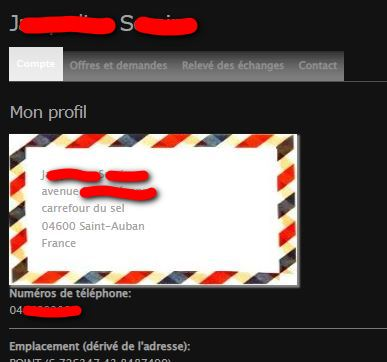
\includegraphics[width=.7\linewidth]{311-page_profil_hors_ligne}
    \caption{Page de profil d'un membre \og hors ligne\fg}
    \label{fig:pageProfilHorsLigne}
\end{figure}

Dans le cas d'un membre \og hors ligne\fg, la page de profil se présente comme à la figure \ref{fig:pageProfilHorsLigne}. L'enveloppe autour de son adresse indique que les seuls messages possibles sont par voie postale ordinaire. Bien que l'onglet \liensmenu{Contact} figure comme sur la page de profil des autres membres, si vous essayez d'envoyer un message (électronique) à ce membre, un petit texte vous préviendra que: \noncliquables{Jxxxx Sxxxxx est un utilisateur sans internet qui n'a pas désigné de représentant. Votre courriel pourrait ne pas recevoir de réponse!}. Sauf si le membre a désigné un représentant --- une adhérente du \CdS l'a fait ---, auquel cas le texte sera: \noncliquables{Ce membre sera contacté par un intermédiaire.}.

Le ou les numéro(s) de téléphone sont néanmoins disponibles pour un contact téléphonique.
\index{fiche de profil!membre hors ligne|(}

\section{Profil complet de Charlotte}
\index{fiche de profil|(}

De nombreuses captures d'écran de ce document ont été prises alors que le profil de Charlotte n'était pas complet. Il comportait seulement les informations indispensables pour créer un compte \CF, un prénom et une adresse courriel (celle qu'on voit sur certaines figures \texttt{charlotte.arnaud2@monfai.xyz} est fantaisiste). À la page suivante, vous trouverez son profil correctement rempli.

\begin{figure}
    \centering
    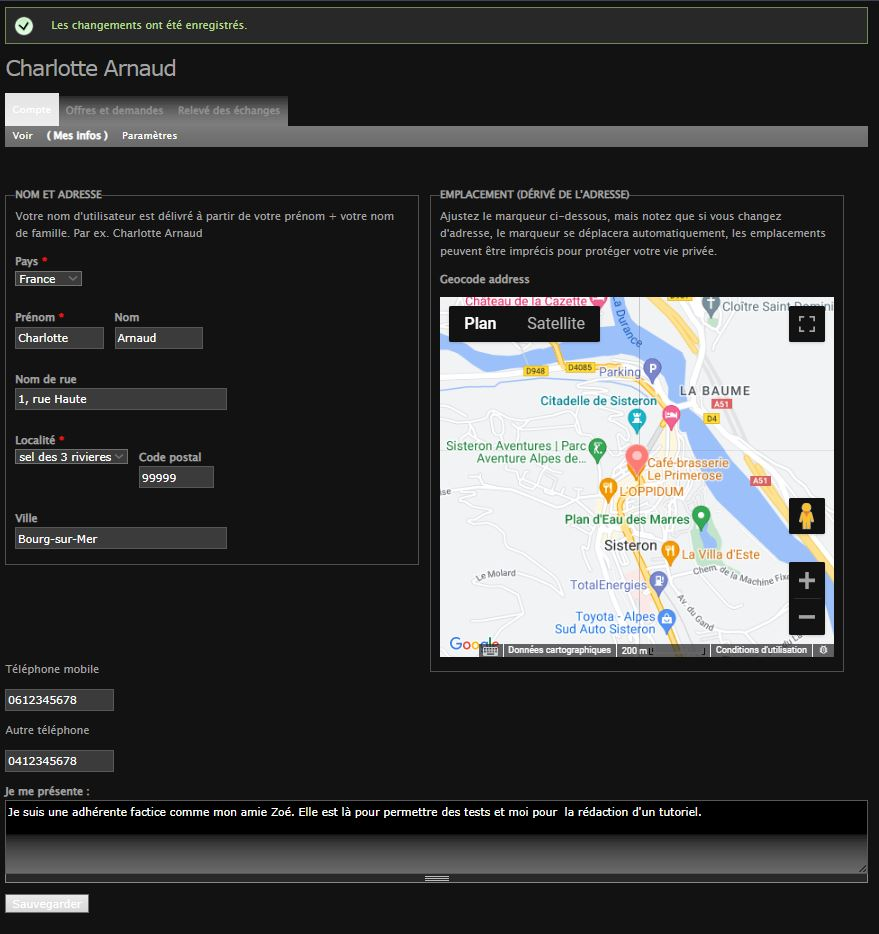
\includegraphics[width=\linewidth]{300-profil_charlotte_complet}
    \caption[Profil complet de Charlotte \textsc{Arnaud}]{Profil complété, onglet <<~Mes infos~>>, de Charlotte \textsc{Arnaud} notre adhérente factice  (l'adresse de Bourg-sur-Mer étant fantaisiste, le positionnement sur la carte est resté à Sisteron !)}
    \label{fig:profilCharlotteComplet}
\end{figure}
\index{fiche de profil|)}

\section{Nouveaux documents}
\label{sec:nouveauxDocuments}
\index{Docs|(}

\begin{figure}
    \centering
    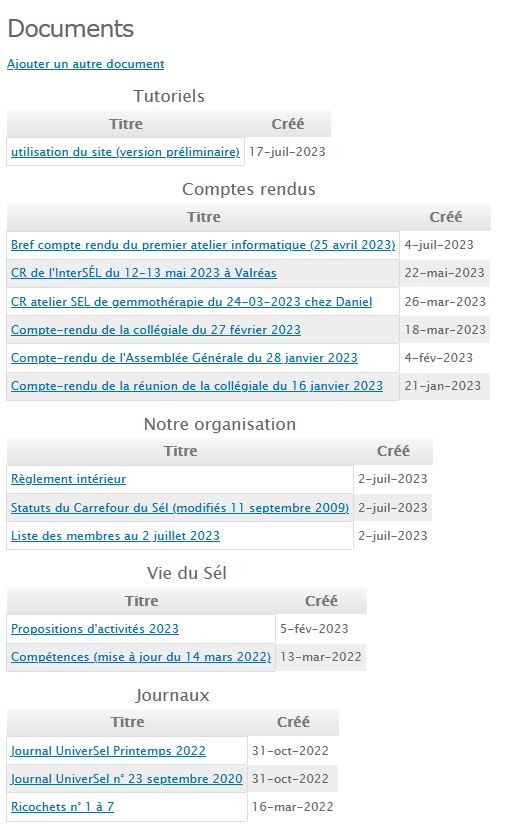
\includegraphics[width=.8\linewidth]{400-documents_au_17_juillet_2023}
    \caption{Liste des documents mise à jour au \oldstylenums{17} juillet \oldstylenums{2023}}
    \label{fig:nouveauxDocuments}
\end{figure}

Depuis la capture d'écran du mois de juin dernier (Fig. \ref{fig:listeDocuments}, p. \pageref{fig:listeDocuments}), j'ai ajouté quelques documents à la rubrique \og Docs \fg du site, voir à la figure \ref{fig:nouveauxDocuments} (p. \pageref{fig:nouveauxDocuments}) la liste mise à jour au \oldstylenums{17} juillet \oldstylenums{2023}.

Y sont ajoutés:
\begin{itemize}
    \item Le compte-rendu que j'avais promis mais pas encore rédigé de l'atelier informatique du \oldstylenums{25} avril dernier.
    \item Les documents officiels de notre \sel: statuts et règlement intérieur.
    \item La liste des membres au \oldstylenums{2} juillet dernier (la dernière pour l'instant). Il s'agit de la liste au format \termecode{pdf} que vous pouvez télécharger et imprimer. Elle comporte tous les numéros de téléphone. Notez que vous pouvez créer cette liste vous même en cliquant sur le lien \autresliens{Version imprimable} de la page \og Membres\fg (voir Fig. \ref{fig:pageMembres} p. \pageref{fig:pageMembres}); ici elle est présentée \og prête à l'emploi\fg pour vous simplifier les choses.
    \item Enfin, j'ai ajouté une version préliminaire du présent tutoriel.
\end{itemize}
\index{Docs|)}
